\documentclass[border=10pt]{standalone}
\usepackage{pgfplots}
\pgfplotsset{compat=1.18}
\begin{document}
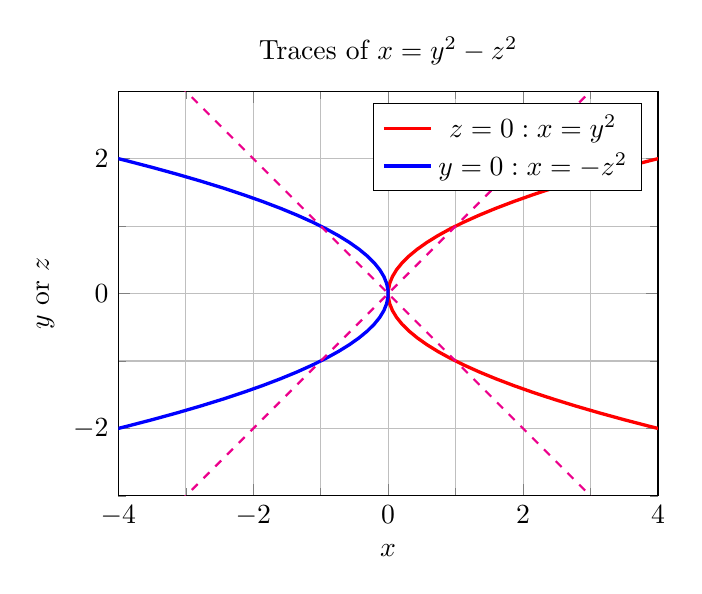
\begin{tikzpicture}
\begin{axis}[
    axis equal image,
    xlabel={$x$}, ylabel={$y$ or $z$},
    title={Traces of $x=y^2-z^2$},
    xmin=-4, xmax=4, ymin=-3, ymax=3,
    samples=100,
    legend pos=north east,
    grid=both,
    minor tick num=1
]
\addplot[red, very thick] ({x^2},{x});
\addlegendentry{$z=0: x=y^2$}
\addplot[blue, very thick] ({-x^2},{x});
\addlegendentry{$y=0: x=-z^2$}
\addplot[magenta, thick, dashed] ({x},{x});
\addplot[magenta, thick, dashed] ({x},{-x});
\end{axis}
\end{tikzpicture}
\end{document}
